\chapter{Ön İnceleme}

Teknolojinin ilerlemesi kullandığımız elektronik aletlerin donanımlarında da olumlu bir değişim sağlamıştır. 10 yıl öncesine ait bir telefondaki donanım, telefon üzerinde yapabileceğimiz işlemleri kısıtlamaktaydı. Günümüz telefonlarında bulunan donanımlar ise telefonları sadece karşı taraf ile iletişim kurmaktan öteye taşımaktadır. Bahsettiğimiz bu akıllı telefonların sahip olduğu gelişmiş işlemciler ve içerdiği ekstra donanımlar, dokunmatik ekran, sensörler, araştırmacılara yeni çalışma alanları sunmaktadır. 
Bu çalışma alanlarından bir tanesi de etkinlik tanımadır (Activity Recognition). Ulaşım türü tespiti ise etkinlik tanımanın alt çalışma alanlarından bir tanesidir. Literatür incelendiğinde ulaşım türü tespiti hakkında yapılmış birçok çalışma olduğu görülmektedir.

Yapılan çalışmalardan bir tanesinde \cite{reddy2008determining} akıllı telefonların GPS ve ivmeölçer algılayıcılarından elde edilen veriler ile ulaşım türü tespiti gerçekleştirilmiştir. Çalışmada aşağıda belirtilen 5 farklı ulaşım türünün tespit edilmesi hedeflenmiştir.\begin{itemize}
  \item Hareketsiz
  \item Yürüme
  \item Koşma
  \item Bisiklet sürme
  \item Motorlu taşıtlar
\end{itemize}

\begin{table}[!h]
\centering
\caption{Sınıflandırıcılara ait doğruluk sonuçları }
\label{my-label}
\begin{tabular}{|l|l|l|l|l|l|l|}
\hline
     & Still & Walk & Run  & Bike  & Motor & All  \\ \hline
NB   & 96.0  & 87.1 & 98.4 & 61.2  & 93.6  & 87.2 \\ \hline
DT   & 98.2  & 96.2 & 98.6 & 91.2  & 94.3  & 95.7 \\ \hline
kNN  & 97.5  & 95.2 & 98.4 & 91.0  & 91.2  & 94.7 \\ \hline
SVM  & 97.8  & 95.6 & 98.2 & 86.9  & 88.4  & 93.4 \\ \hline
CHMM & 96.2  & 96.1 & 98.4 & 89.4, & 91.7  & 94.4 \\ \hline
\end{tabular}
\end{table}

Tablo 2.1'de çalışmanın 5 farklı makine öğrenmesi algoritmasına ait doğruluk değerleri bulunmaktadır. Çalışmada sınıflandırma algoritması olarak Decision Tree (Karar Ağacı) kullanılmıştır. Sensör verileri toplanırken mobil cihaz cepte taşınmıştır. 
\newpage

%\begin{figure}[!htbp]
%\centering
%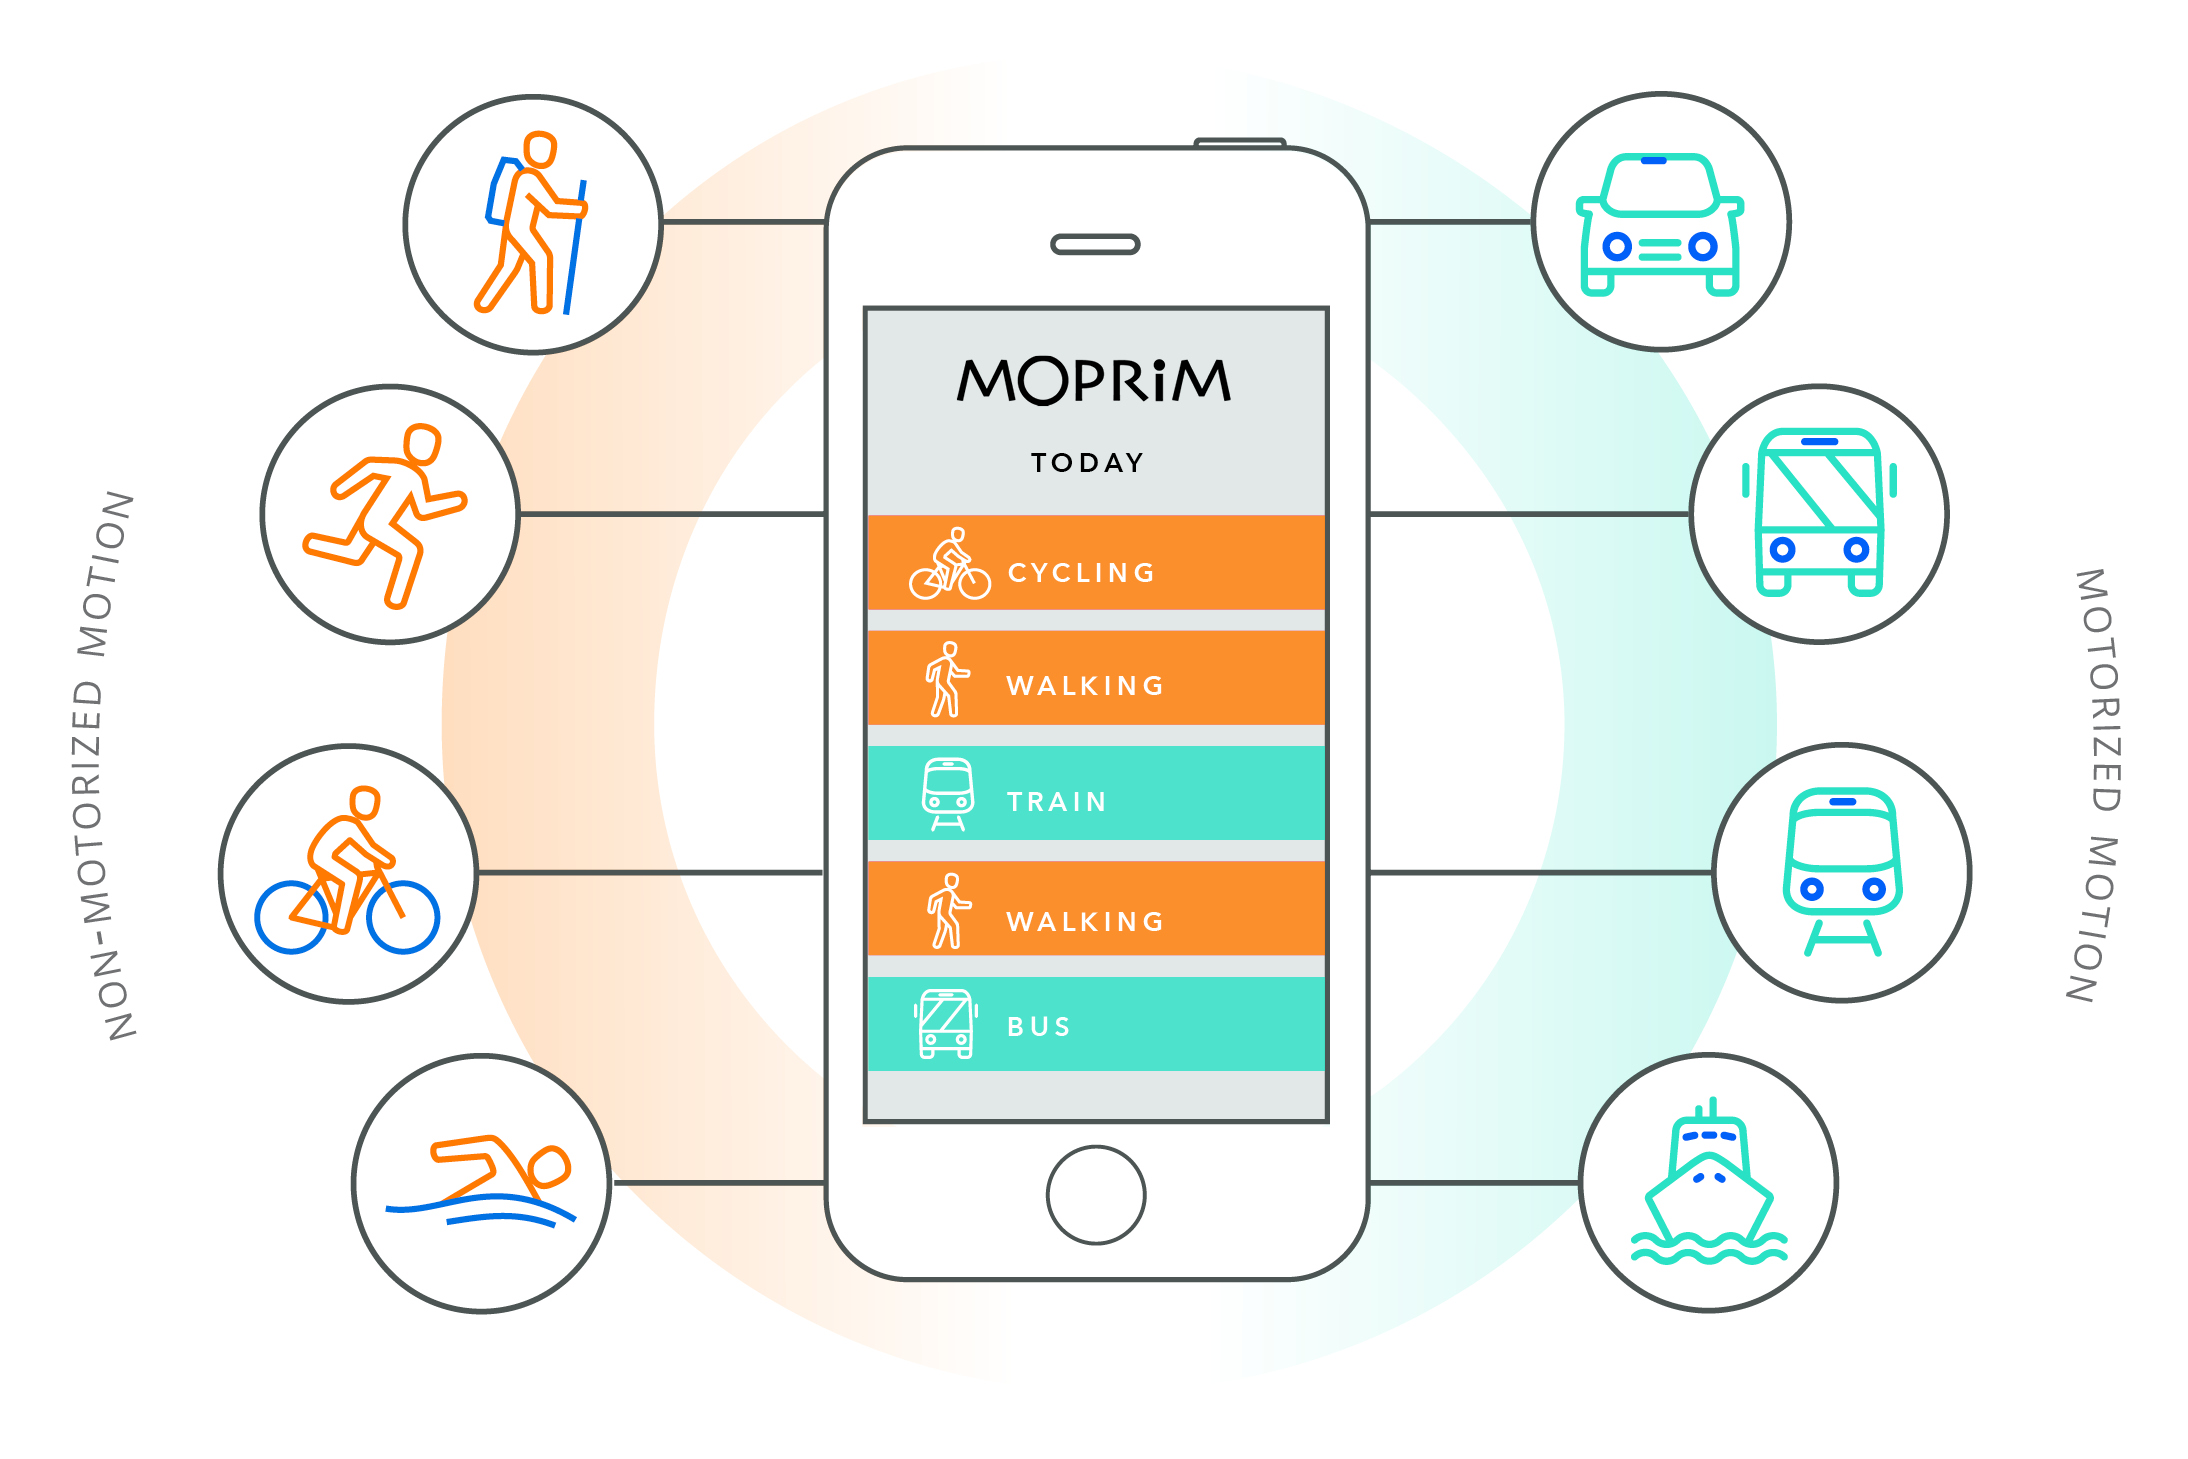
\includegraphics[scale=0.3]{projectChapters/images/illustration-moprim-2.jpg}
%\caption{Etkinlik tanıma örnek uygulama}
%\end{figure}
%Bu işlem kabaca kullanıcının aktivitelerinin, kullandığı akıllı telefonun sensörlerine dayalı olarak elde edilmesi işlemidir. Etkinlik tanıma bir çok alt çalışma alanına sahiptir. Örnek vermek gerekirse, kullanıcıların sağlık bilgilerinin görüntülenmesini amaçlayan health monitoring, öneri sistemleri (recomendation systems) ve kullanıcı davranış analizi (study of personal behavior). Bu projede ise etkinlik tanımanın alt dallarından ulaşım türü tespiti (transporting mode) üzerinde durulmuştur. 

%\begin{figure}[!htbp]
%\centering
%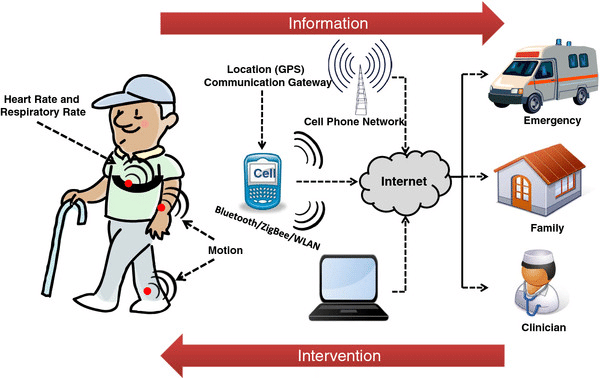
\includegraphics[scale=0.4]{projectChapters/images/health.png}
%\caption{Health monitoring çalışma sistemi}
%\end{figure}

%Ulaşım türü tespiti konusunda şimdiye kadar yapılmış birçok çalışma bulunmaktadır. Yapılan çalışmalar iki ayrı alandan oluşmaktadır. Bir tanesinde kullanıcının hareketleri esas alınmakta yani sensor verileri yürüme, oturma, kalkma, koşma vb. alt alanlar üzerinden sınıflandırılır \cite{bayat2014study}. Bu çalışma alanı akıllı telefonların yanı sıra günümüzün yeni teknolojisi akıllı saatlerde de  sıkça kullanılmaktadır. Özellikle spor odaklı yazılımlar bu sistemi kullanarak kullanıcının ne kadar süre koştuğu veya ne kadar süre yürüdüğü gibi bilgileri sensörlerden elde ederek kullanıcıya sunmaktadır.



Wang S. , Chen C  ve Ma J. tarafından yapılan çalışmada \cite{wang2010accelerometer} akıllı telefonlarda bulunan algılayıcılardan sadece dâhili ivmeölçeri kullanarak ulaşım türü tespit edilmiştir. Çalışmada aşağıda belirtilen 6 farklı ulaşım türünün tespit edilmesi hedeflenmiştir.\begin{itemize}
  \item Hareketsiz
  \item Yürüme
  \item Bisiklet sürme
  \item Otobüs
  \item Araba
  \item Metro
\end{itemize}

GPS teknolojisinin çok fazla enerji tüketmesi nedeniyle çalışmada kullanılmamıştır. Ayrıca GPS sensörleri yer altında veri toplayamamaktadır. Böylece metro gibi yer altından giden araçlar tespit edilememektedir.



Sökün H. , Kalkan H. ve Cetişli B. \cite{sokun2012classification}, tarafından yapılan çalışmada üç eksenli ivmeölçerden alınan sinyaller kullanılarak temel fiziksel hareket sınıflandırılması yapılmıştır. Geliştirilen yöntem ile ivmeölçeri taşıyan insanın araç ile mi, yoksa yaya olarak mı seyahat ettiğinin tespit edilmesi amaçlanmıştır. Alınan veriler belirli zaman aralıklarında incelenmiş ve gerçek zamanlı olarak kNN (k En Yakın Komşu) algoritması kullanılarak sınıflandırılmıştır.


Feng ve Timmermans \cite{feng2013transportation} GPS ve ivmeölçer verileri kullanarak ulaşım türü tespiti gerçekleştirmiştir. Yapılan çalışmada üç farklı yöntem incelenmiştir.
\begin{itemize}
  \item Sadece GPS verisi kullanarak sınıflandırma
  \item Sadece İvmeölçer verisi kullanarak sınıflandırma
  \item GPS ve ivmeölçer verisi kullanarak sınıflandırma
\end{itemize}

Sadece ivmeöçler verisi kullanılarak yapılan tahminler sadece GPS verisi kullanarak yapılan tahminlerden daha iyi performans sergilemiştir. GPS ve ivmeölçer verilerini birleştiren yaklaşım ise en iyi performansı vermiştir. Çalışmada sınıflandırma yöntemi olarak Bayes Ağlarık (Bayesian Belief Networ) kullanılmıştır. Proje kapsamında aşağıda belirtilen 6 farklı ulaşım türünün tespit edilmesi hedeflenmiştir.
\begin{itemize}
  \item Yürüme
  \item Koşma
  \item Bisiklet sürme
  \item Motor sürme
  \item Otobüs
  \item Araba
  \item Tramvay
  \item Metro
\end{itemize}


Stenneth ve Wolfson \cite{stenneth2011transportation} telefon ve coğrafi bilgi sistemleri bilgileri ile ulaşım türü tespiti üzerinde çalışmıştır. Çalışma kapsamında aşağıda belirtilen 6 farklı ulaşım türünün tespit edilmesi hedeflenmiştir.
\begin{itemize}
  \item Tren
  \item Hareketsiz
  \item Yürüme
  \item Bisiklet sürme
  \item Otobüs
  \item Araba
\end{itemize}
Toplanan veriler beş (Bayesian Net, Decision Tree, Random Forest, Naïve Bayesian, Multilayer Perceptron) farklı makine öğrenmesi algoritması ile test edilmiştir. En iyi sonucu \%93 doğruluk oranıyla Random Forest algoritması vermiştir.
\newpage

Bu proje kapsamında daha önceden yapılan çalışmalardan farklı olarak ivmeölçerin yanında jiroskop sensörü de kullanılmıştır. İki sensörden toplanan veriler dört farklı makine öğrenmesi algoritmasında test edilip en iyi sonucu veren algoritmaya ait model sınıflandırma işlemi için kullanılmıştır. 
Kullanılan Makine öğrenmesi algoritmaları aşağıdaki gibidir.
\begin{itemize}
  \item Naive Bayes
  \item kNN
  \item J48
  \item Random Forest
\end{itemize}
GPS sensörü fazla enerji tüketmesi ve yer altında veri toplayamaması nedeniyle tercih edilmemiştir.








%\begin{figure}[!htbp]
%\centering
%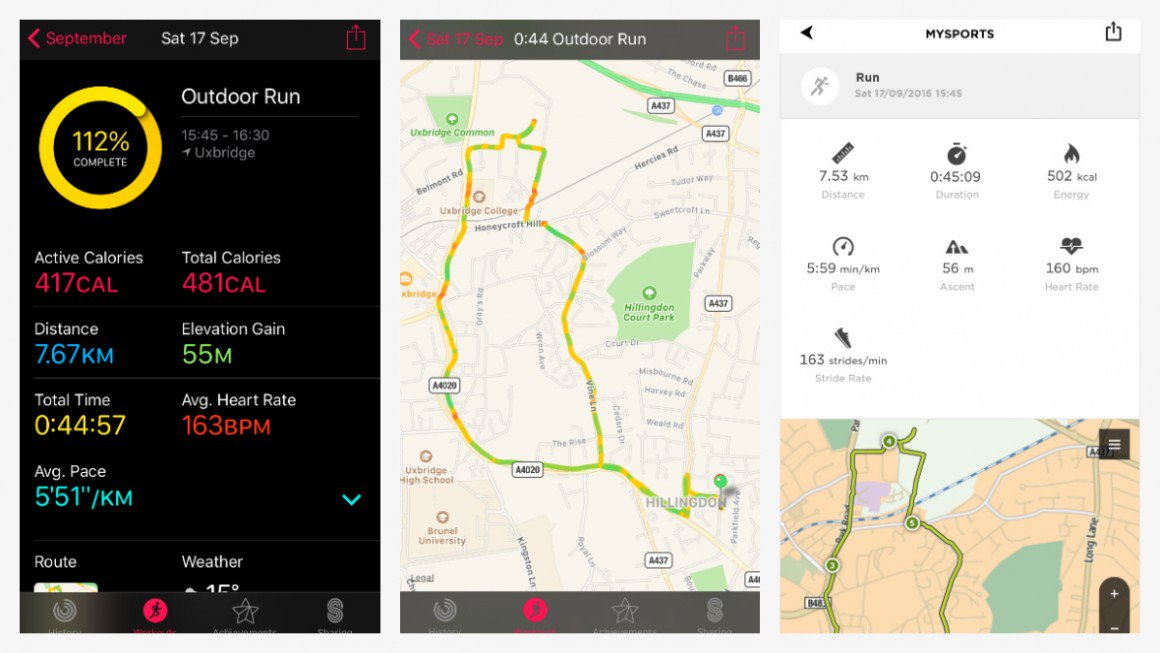
\includegraphics[scale=0.4]{projectChapters/images/activity_recog_app.jpg}
%\caption{Etkinlik tanıma örnek uygulama}
%\end{figure}

%\newpage

%Diğer tarafta ise sensor verileri otobüs, bisiklet, metro vb. kullanıcının kullandığı vasıtalara göre sınıflandırılmaktadır \cite{widhalm2012transport}. Bu proje de kullanıcının kullandığı vasıtalara dayalı bir sınıflandırma yapılmıştır. Fakat sınıflandırma İstanbul sınırlarında bulunan toplu taşımalar ile detaylandırılmıştır. Projede veriler araba, otobüs, metro, metrobüs, marmaray, tramvay ve hafif raylı olmak üzere toplamda 7 ayrı vasıta için sınıflandırılmıştır. Şimdiye kadar ulaşım türü tespitine ait çalışmalarda sınıflandırma bahsedilen vasıtalar kadar detaylı değil daha yüzeyseldir. 

%\begin{figure}[!htbp]
%\centering
%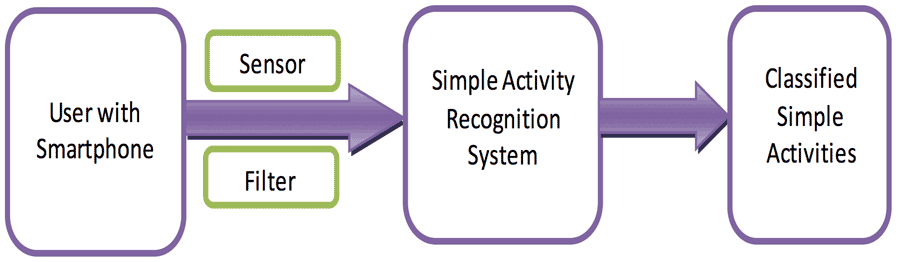
\includegraphics[scale=0.4]{projectChapters/images/Fig1.png}
%\caption{Etkinlik tanıma işlemi ana adımları}
%\end{figure}


%Yapılan çalışmalar incelendiğinde,  akıllı telefonların sadece sensörlerinden faydalanılmadığını, wi-fi sinyalleri ve GPS verilerinin de kullanıldığı görüldü. Fakat GPS verileri ve wi-fi sinyalleri yeraltında örneğin; metro, marmaray gibi vasıtaların kullanıldığı durumlarda doğru bilgiler vermelerinin mümkün olmadığı gerekçesiyle projede kullanılmamıştır. İncelemelerde sensör olarak sadece ivmeölçer kullanılmıştır fakat bu projede ivmeölçer ile birlikte jiroskop kullanılmıştır.
%Sensörlerden elde edilen verilerden  makine öğrenmesi algoritmalarına dayalı bir model oluşturulup bu modele dayalı bir sınıflandırma algoritması kullanılmıştır.
